% !TEX encoding = UTF-8 Unicode
\subsection{Fase A}
	\textbf{Periodo}: dal \insdate{25}{11}{2014} al \insdate{23}{01}{2015} \\
	Questa fase comincia con la presentazione in aula delle “Regole del progetto didattico”. Essa termina con la scadenza della consegna della \insrev{Revisione dei Requisiti}.\\Le sottofasi sono le seguenti:
	\begin{description}
		\item[Individuazione/creazione strumenti]: In questa sottofase vengono scelti gli strumenti che saranno utilizzati per la stesura dei documenti, per il tracciamento dei requisiti e alcuni script di controllo dei documenti. Se alcuni di essi non sono disponibili nella rete o non soddisfacenti, verranno creati su misura.
		\item[Norme di Progetto]: Dopo aver individuato gli strumenti si potrà procedere alla stesura del documento \insfile{Norme Di Progetto 1.0}. Questo documento sarà utilizzato indipendentemente dal capitolato che sarà preso in appalto.
		\item[Creazione documentazione]: In questa fase sappiamo esattamente con cosa e in che modo dobbiamo scrivere un documento e possiamo iniziare la stesura dei documenti.
			\begin{itemize}
				\item \textbf{Studio di Fattibilità}: Vengono valutati pro e contro di tutti i capitolati proposti e viene redatto il documento \insfile{Studio Di Fattibilità 1.0}. Viene quindi scelto il capitolato da sviluppare.
				\item \textbf{Analisi dei Requisiti}: Viene steso il documento \insfile{Analisi Dei Requisiti 1.0}. Prima e durante la stesura di questo documento verranno fatti degli incontri con il proponente per consolidare i requisiti stesi o per chiarire le idee sui requisiti da stendere.
				\item \textbf{Piano di Progetto}: Si stende il documento \insfile{Piano Di Progetto 1.0} per regolare le attività che il team dovrà svolgere.
				\item \textbf{Piano di Qualifica}: Si redige il documento \insfile{Piano Di Qualifica 1.0}.
				\item \textbf{Glossario}: viene incrementato il file  \insfile{Glossario.xml} e steso in modo automatico il documento \insfile{Glossario 1.0}.
			\end{itemize}
	\end{description}
	\subsubsection{Diagramma di Gantt delle attività}
		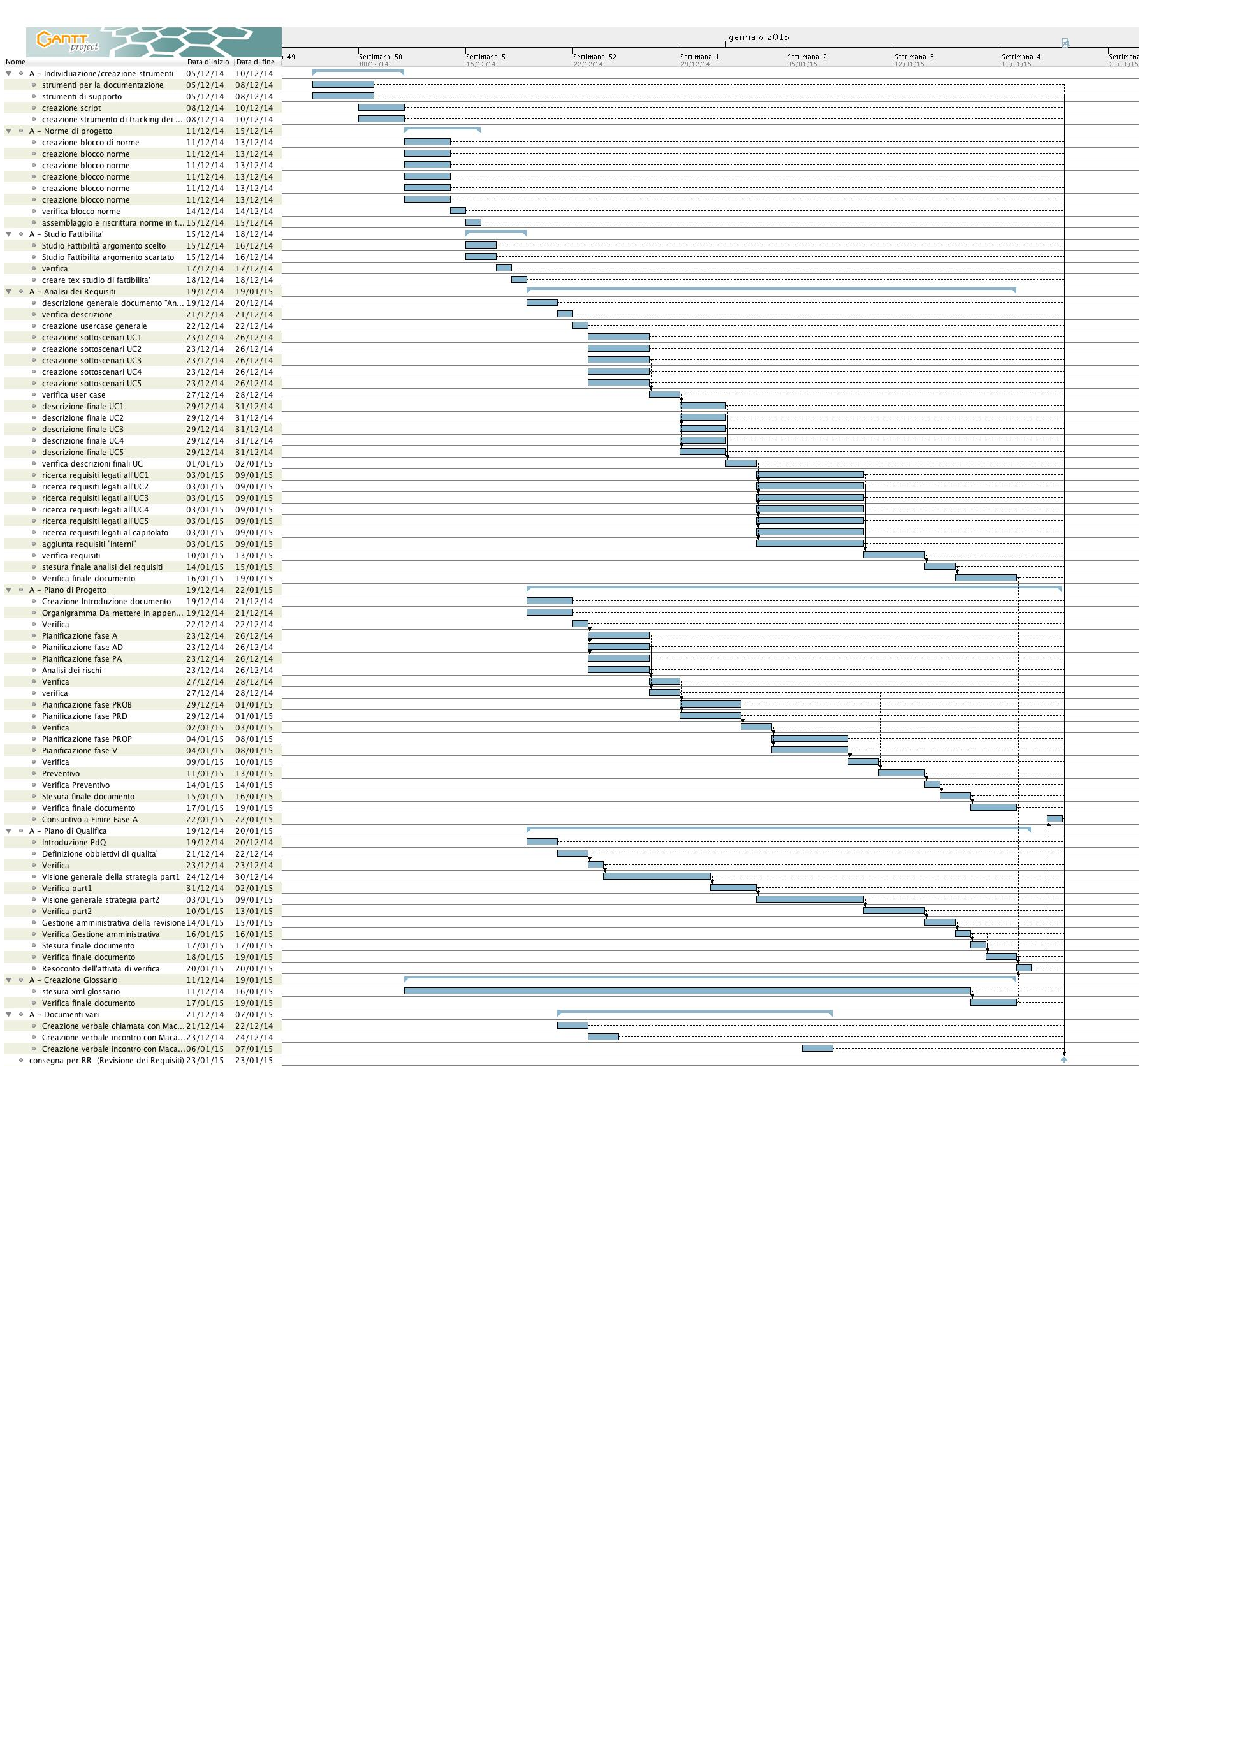
\includegraphics{PianoDiProgetto/Pics/FaseA.pdf}
